\documentclass{standalone}
\usepackage{tikz}
\begin{document}
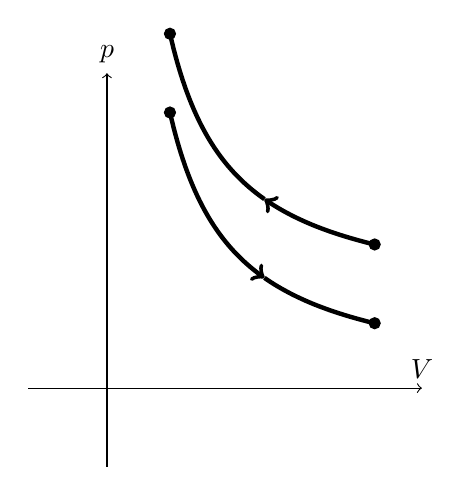
\begin{tikzpicture}[scale=2]
    \draw[->](0,-0.5)--(0,2)node[above]{$p$};
    \draw[->](-0.5,0)--(2,0)node[above]{$V$}; 
    \draw[->,ultra thick]plot[smooth,domain=0.4:1](\x,{0.7/(\x)});   
    \draw[-,ultra thick]plot[smooth,domain=1:1.7](\x,{0.7/(\x)});
    \draw[-,ultra thick]plot[smooth,domain=0.4:1](\x,{0.5+0.7/(\x)});   
    \draw[<-,ultra thick]plot[smooth,domain=1:1.7](\x,{0.5+0.7/(\x)});

    \filldraw[black](1.7,0.912)circle(1pt);
    \filldraw[black](1.7,0.412)circle(1pt);
    \filldraw[black](0.4,2.25)circle(1pt);
    \filldraw[black](0.4,1.75)circle(1pt);
\end{tikzpicture}
\end{document}